%\documentclass[preprint, review, 3p, authoryear]{elsarticle}
\documentclass[10pt, a4paper]{article}

%\usepackage{setspace}
\usepackage[utf8]{inputenc}
\usepackage{amsmath, amssymb, amsthm, bbm}
\usepackage{xcolor}
\usepackage{graphicx}
\usepackage[authoryear]{natbib}
\usepackage{apalike}
\usepackage{relsize}
\usepackage{array}
\usepackage{multirow}
\usepackage{showlabels}
\usepackage{setspace}

\DeclareMathOperator*{\argmax}{arg\,max}

\newtheorem{prob}{Problem}
\newtheorem{prop}{Proposition}
\newtheorem{definition}{Definition}

%%%%% bold symbol in math enviornment
\newcommand{\m}[1]{\boldsymbol{#1}}

\title{Merging the components of a finite mixture using  posterior probabilities}
\author{M. Comas-Cufí \and J.A. Martín-Fernández \and G. Mateu-Figueras}

%\doublespacing
\begin{document}

\maketitle

\section{Introduction}

%Cl
The most standard parametric approach in cluster analysis assumes data can be modelled by a finite mixture distribution. The approach has two steps; first, a finite mixture distribution with probability density function
\[
f(\;\cdot\; ; \pi_1, \dots, \pi_k, \m\theta_1 \dots \m\theta_k) = \pi_1   f(\;\cdot\; ; \m\theta_1) + \dots + \pi_k f(\;\cdot\; ; \m\theta_k),
\]%
%with $\sum_{j=1}^k = \pi_j =1$
is fitted to a sample $\m X$, obtaining estimates $\hat{\pi}_1, \dots, \hat{\pi}_k$ and $\hat{\m\theta}_1 \dots \hat{\m\theta}_k$. Second, after the fitting process, each observation $\m x$ is assigned to the finite mixture component $j$, $1\leq j \leq k$, with $\hat{\pi}_j f(\m x ; \hat{\m\theta}_j)$ maximum.

In the previous approach, it is common to have mixture components not separated enough from other mixture components, and therefore, it is difficult to consider them as two different clusters. To deal with this situation, different authors propose to consider clusters formed by two or more components. Therefore, the crucial point here is to combine or to merge different components into one single one ({\color{red} Cites rellevants per el problema d'ajuntar components. Preparar llista actualitzada i afegir les cites segons la revista on es decideixi enviar}).

In this paper we review different approaches that we can find in the literature to combine the finite mixtures components. All methods described in this paper are based on posterior probabilities, $\hat{\tau}_{ij}$, that an observation $\m x_i$, $1\leq i \leq n$, is generated by component $j$, $1\leq j\leq k$. A new approach based on log-ratios to introduce a compositional analysis for the posterior probability vector is also presented. Although this approaches have been presented for Gaussian mixtures \citep{longford2014,melnykov2013distribution,hennig2010methods,baudry2010combining}, the fact that they are based only on the posterior probabilities allow us to apply each method using any other probability distribution mixtures.

Finally, using a generic definition, an integrated formulation to unify such merging methods is presented and discussed. We show that this new formulation opens the way to define new methods based on the posterior probabilities.

The paper is organised as follows: In Section~\ref{definitions} we introduce two concepts; \emph{the partition of a finite mixture distribution} and \emph{the hierarchical combination of components}. The definitions are going to be useful to standardise notation between different methods. In the same section, we show a simple example to get used to the new notation. In Section~\ref{old_methods}, the approaches to obtain a hierarchical combination of components appeared in \cite{hennig2010methods} and \cite{baudry2010combining} are presented using the new notation. In the same section some new proposals are introduced. One of the new approaches is based on \cite{longford2014}, the other ones are build considering the geometric nature of the posterior probabilities i.e using the log-ratio approach. In Section~\ref{confusion} the integrated formulation to unify the methods is presented. In Section~\ref{comparison} a comparison of the different approaches is done using simulated data sets. Finally, Section~\ref{conclusions} contains the conclusions and final remarks.

\section{Definitions}
\label{definitions}

Let $\mathbb{X}$ be a sample space. A \emph{finite mixture of distributions} is a probability distribution with probability density function (pdf) defined as the linear combination of pdf from other probability distributions defined in $\mathbb{X}$. In general, the pdf $f$ of a finite mixture of distributions is
\begin{equation}\label{mixt}
f(\;\cdot\; ; \pi_1, \dots, \pi_k, \m\theta_1 \dots \m\theta_k) = \pi_1 f_1(\;\cdot\; ; \m\theta_1) + \dots + \pi_k f_k(\;\cdot\; ; \m\theta_k),
\end{equation}
where $\m\theta_1, \dots,  \m\theta_k$ are the parameters of the pdf $f_1, \dots, f_k$ respectively and, because $\int_{\mathbb{X}}f = 1$ the restriction $\sum_{\ell = 1}^k \pi_\ell = 1$ holds. The pdf's $f_1, \dots, f_k$ are called the \emph{components} of the finite mixture $f$, or simply the \emph{mixture components}.

Let $f$ be a finite mixture of distributions with  parameters  $\pi_1, \dots, \pi_k, \m\theta_1 \dots \m\theta_k$ as defined in Equation~\ref{mixt}, and let $I$  be a subset of $\{1, \dots, k\}$. We denote by $f_I$ the finite mixture of distributions with pdf defined by
\[
f_I = \sum_{j \in I} \frac{\pi_i}{\pi_I} f_j(\;\cdot\; ; \m\theta_j)
\]
where $\pi_I = \sum_{\ell \in I} \pi_\ell$. To simplify, we do not specify the parameters of $f_I$, which are parameters borrowed from $f$. Note that using this notation, we have the particular cases $f_{\{1, \dots, k\}} = f$ and $f_{\{j\}} = f_j$.

A \emph{partition} $\mathcal{I}$ of $\{1, \dots, k\}$ is a set of subsets of $\{1, \dots, k\}$, called $parts$, such that $\bigcup_{I \in \mathcal{I}} I = \{1, \dots, k\}$ and  if two parts $I, J \in \mathcal{I}$ are different, $I \cap J = \emptyset$ holds. To simplify, through this paper we assume an order within the elements of a partition. Doing so, we can index the partition and write $\mathcal{I} = \{ I_1, \dots, I_s\}$. It is important to note that given any partition $\mathcal{I} = \{ I_1, \dots, I_s\}$ of $\{1, \dots, k\}$, the mixture $f$ (Eq.~\ref{mixt}) can be rewritten as
\begin{equation}
f = \pi_{I_1} f_{I_1} + \dots + \pi_{I_s} f_{I_s}.
\label{mixt_part}
\end{equation}


A \emph{hierarchical combination of components} is a sequence of partitions $\mathcal{I}_1, \dots, \mathcal{I}_k$ of $\{1,...,k\}$, where $\mathcal{I}_1$ is the one-part partition $\mathcal{I}_1 = \{ \{1, \dots, k\} \}$, and for each $k'$, $1 <  k' \leq k$,
\begin{itemize}
\item $\mathcal{I}_{k'}$ has $k'$ elements  and
\item if a part $I \in \mathcal{I}_{k'-1}$ then either there is a part $J \in \mathcal{I}_{k'}$ with $J = I$ or there are two parts $J_1, J_2 \in \mathcal{I}_i$ with $I = J_1 \cup J_2$.
\end{itemize}

{\color{blue} jo aqu\'{\i} potser ho resumiria amb una frase on es digui que a cada nova partició s'agafa un dels subsets de la partició anterior i es parteix en dos (és així, no?)}

\subsection*{Model-based clustering}
{\color{blue} Jo potser unificaria la notació de la mostra. Diria $X = \{\m x_1\dots, \m x_n\}$ i utilitzaria $\m x_i$ i $\m x_j$. En gaireb\'{e} tot l'article ho fas servir per\`{o} en aquesta part utilitzes $\m x$ i $\m y$. Pensa't tamb\'{e} la notaci\'{o} de $\hat{f}_{I_{j^*}}$, vull dir el hat sobre les fs de l'equaci\'{o} 3, li poses per indicar que \'{e}s la mixtura amb els par\`{a}metres estimats?.}

When model-based clustering is based on finite mixtures, a common approach is to assume that a given sample follows a finite mixture of distributions $f_1, \dots, f_k$, and then to proceed as follows,
\begin{enumerate}
\item to find a suitable estimators $\hat{\pi}_1, \dots, \hat{\pi}_k,$ $\hat{\m\theta}_1, \dots, \hat{\m\theta}_k$ of parameters $\pi_1, \dots, \pi_k,$ $\m\theta_1, \dots, \m\theta_k$, and
\item to classify each observation according to the maximum posteriori criteria, i.e., two observations $\m x, \m y \in \mathbb{X}$ are classified to same cluster if and only if
\[
\argmax_{j=1}^k \frac{ \hat{\pi}_j f_j(\m x ; \hat{\m\theta}_j) }{\sum_{\ell=1}^k \hat{\pi}_\ell f_\ell(\m x ; \hat{\m\theta}_\ell) } = \argmax_{j=1}^k \frac{ \hat{\pi}_j f_j(\m y ; \hat{\m\theta}_j) }{ \sum_{\ell=1}^k \hat{\pi}_\ell f_\ell(\m y ; \hat{\m\theta}_\ell) }.
\]
\end{enumerate}


\cite{lee2004combining,hennig2010methods,baudry2010combining,melnykov2013distribution,pastore2013merging} noted that associating one mixture component to one cluster can be misleading, because different mixture components can be not separated enough to be considered as a unique cluster. For example, Figure~\ref{ex_mixture} shows  a mixture with 6 Gaussian components adjusted to a dataset. The standard approach is to associate one cluster to one mixture component, ending up with 6 clusters. Instead, they proposed that one cluster can be formed by the combination of different mixture components.

We use the notation of partitions introduced previously to formalise the proposal of considering different mixture components as one cluster. We define the clustering defined by a partition as follows: given a partition $\mathcal{I} = \{ I_1, \dots, I_s\}$, two elements $\m x, \m y \in \mathbb{X}$ are classified to the same cluster if and only if
\begin{equation}\label{cluster_criteria}
\argmax_{j=1}^s \frac{ \hat{\pi}_{I_j} \hat{f}_{I_j}(\m x) }{\sum_{\ell=1}^s \hat{\pi}_{I_\ell} \hat{f}_{I_\ell}(\m x ) } = \argmax_{j=1}^s \frac{ \hat{\pi}_{I_j} \hat{f}_{I_j}(\m y) }{ \sum_{\ell=1}^s \hat{\pi}_{I_\ell} \hat{f}_{I_\ell}(\m y) }
\end{equation}
where $\hat{f}_{I_j}(\;\cdot\;) = \sum_{j' \in I_j} \frac{\hat{\pi}_{j'}}{\hat{\pi}_{I_j}} f_{j'}(\;\cdot\; ; \hat{\m\theta}_{j'})$ and $\hat{\pi}_{I_j} =  \sum_{j' \in I_j} \hat{\pi}_{j'}$. To be more specific,  if for $\m x \in \mathbb{X}$ we have
\[
j^* = \argmax_{j=1}^s \frac{ \hat{\pi}_{I_j} \hat{f}_{I_j}(\m x) }{\sum_{\ell=1}^s \hat{\pi}_{I_\ell} \hat{f}_{I_\ell}(\m x ) },
\]
we say that the element $\m x$ is classified to part $I_{j^*}$. Equivalenty, we also say that element $\m x$ is classified to component $\hat{f}_{I_{j^*}}$.

Finally, because all methods presented in this articles are based on the posterior probabilities, we introduce some notation to facilitate the exposition:


Let $X = \{\m x_1\dots, \m x_n\}$ be a sample defined in $\mathbb{X}$. Given a partition $\mathcal{I} = \{ I_1, \dots, I_s \}$ the posterior probability  of $\m x_i$ being classified to $I_j$ is
\[
\hat{\tau}_{i I_j} =  \frac{ \hat{\pi}_{I_j} \hat{f}_{I_j}(\m x_i) }{\sum_{\ell=1}^s \hat{\pi}_{I_\ell} \hat{f}_{I_\ell}(\m x_i)},
\]
and, for a partition  $\mathcal{I} = \{ I_1, \dots, I_s\}$, we define the posterior probability vector as
\[
\hat{\tau}_{i \mathcal{I}} = \left( \hat{\tau}_{i I_1} , \dots, \hat{\tau}_{i I_s}  \right).
\]
Note that whenever  $\mathcal{I} = \{ I_1, \dots, I_s\}$ is a partition, $\sum_{j=1}^s \hat{\tau}_{i I_j} = 1$ for $1 \leq i \leq n$.

{\color{blue} Estic dubtant de si parlar de la matriu de posterioris, \'{e}s a dir, indicar que en el fons treballarem amb una matriu on cada fila indica un element de la mostra i cada columna el posteriori d'estar classificat a cada $I_j$. Potser despr\'{e}s ser\`{a} m\'{e}s senzill explicar de forma intu\"{\i}tiva cada m\`{e}tode???}

\subsection*{An example using a mixture with 6 components}
{\color{blue} jo veig m\'{e}s l\`{o}gic dir primer com has simulat la mostra i llavors com l'has ajustat amb una mixtura de 6.}

For the sake of an example consider the following estimated Gaussian mixture

\[
\hat{f} = \sum_{j=1}^6 \hat{\pi}_j \phi(\;\cdot\; ; \hat{\m\mu}_j, \hat{\m\Sigma}_j)
\]
with parameters
{\small
\[
\begin{array}{l@{\hskip 0.1in}l@{\hskip 0.1in}c }
\hat{\pi}_1 = 0.13, & \hat{\m\mu}_1 = \left(10.8,69.17\right), & \hat{\m\Sigma}_1 = \left(
\begin{array}{cc}
36.41&1.45 \\ 
1.45&55.13 \\ 
\end{array}
\right), \\ & &\\ 
\end{array}
\]
\[
\begin{array}{l@{\hskip 0.1in}l@{\hskip 0.1in}c }
\hat{\pi}_2 = 0.09, & \hat{\m\mu}_2 = \left(32.68,22.46\right), & \hat{\m\Sigma}_2 = \left(
\begin{array}{cc}
26.76&1.07 \\ 
1.07&40.52 \\ 
\end{array}
\right), \\ & &\\ 
\end{array}
\]
\[
\begin{array}{l@{\hskip 0.1in}l@{\hskip 0.1in}c }
\hat{\pi}_3 = 0.07, & \hat{\m\mu}_3 = \left(13.65,51.91\right), & \hat{\m\Sigma}_3 = \left(
\begin{array}{cc}
33.95&1.35 \\ 
1.35&51.39 \\ 
\end{array}
\right), \\ & &\\ 
\end{array}
\]
\[
\begin{array}{l@{\hskip 0.1in}l@{\hskip 0.1in}c }
\hat{\pi}_4 = 0.16, & \hat{\m\mu}_4 = \left(83.8,4.21\right), & \hat{\m\Sigma}_4 = \left(
\begin{array}{cc}
82.27&3.28 \\ 
3.28&124.56 \\ 
\end{array}
\right), \\ & &\\ 
\end{array}
\]
\[
\begin{array}{l@{\hskip 0.1in}l@{\hskip 0.1in}c }
\hat{\pi}_5 = 0.24, & \hat{\m\mu}_5 = \left(41.28,19.51\right), & \hat{\m\Sigma}_5 = \left(
\begin{array}{cc}
55.87&2.23 \\ 
2.23&84.59 \\ 
\end{array}
\right), \\ & &\\ 
\end{array}
\]
\[
\begin{array}{l@{\hskip 0.1in}l@{\hskip 0.1in}c }
\hat{\pi}_6 = 0.32, & \hat{\m\mu}_6 = \left(24.69,66.04\right), & \hat{\m\Sigma}_6 = \left(
\begin{array}{cc}
57.85&2.3 \\ 
2.3&87.58 \\ 
\end{array}
\right), \\ & &\\ 
\end{array}
\]

}

The mixture $\hat{f}$ with $6$ components was obtained as follows:
\begin{enumerate}
\item A sample  $X_{500}=\{\m x_1, \dots, \m x_{500}\}$ was generated from a Gaussian mixture \emph{with 3 components}. The generation was done using the R package \textsc{MixSim}. The overlapping between components $\omega$ is a measure that defined the overlapping between components in a mixture (see Melnykov for more details). To generate sample $X_{500}$ a maximum overlapping $\check{\omega} = 0.01$ was fixed. {\color{blue} Marc aquest s\'{\i}mbol sobre la omega vol dir alguna cosa?}
\item A Gaussian mixture \emph{with 6 components} was fitted to sample $X_{500}$. To fit the finite mixture the R package \textsc{Rmixmod} was used.
\end{enumerate}
In Figure~\ref{ex_mixture} the sample $X_{500}$ is represented with the isodensity curves of the adjusted mixture $\hat{f}$. The estimated parameter $\hat{\mu}_j$ of each component is represented by a cross.

\begin{figure}[thbp]
\begin{center}
\begin{tabular}{cc}
 %   6 toy mixture
  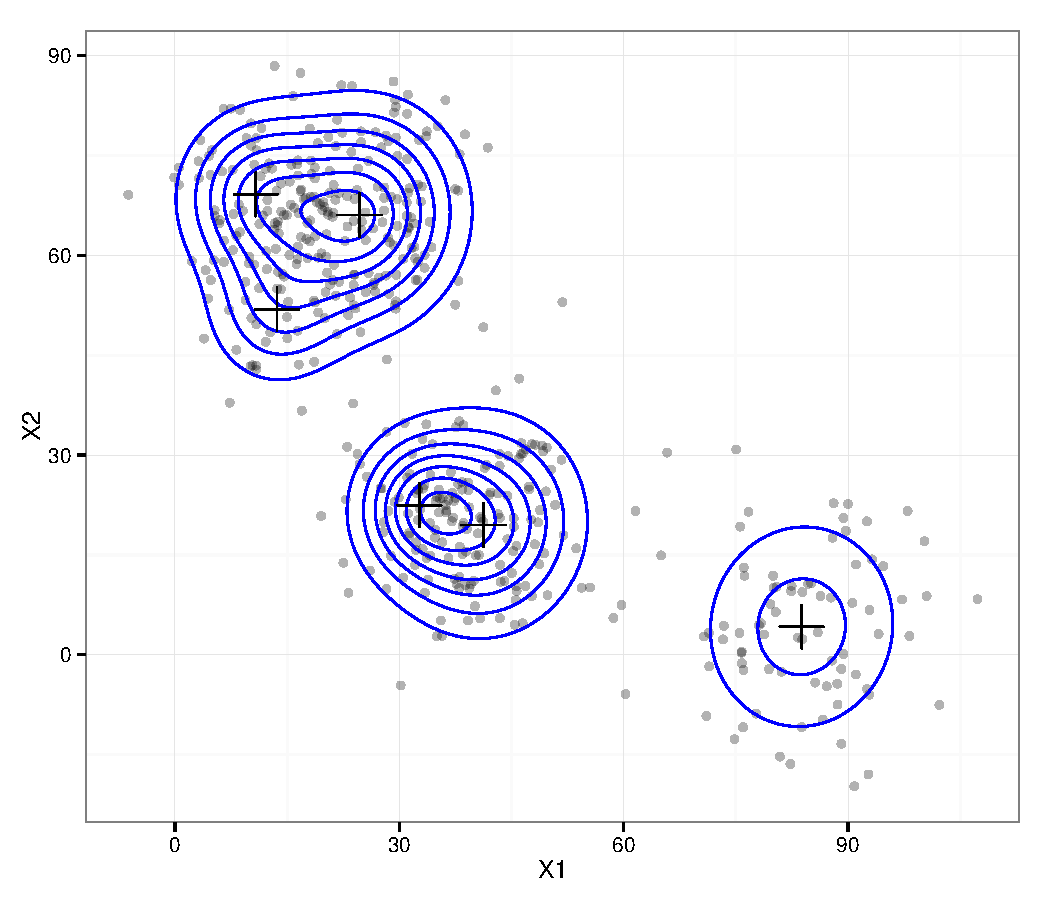
\includegraphics[trim=0cm 0cm 0cm 0cm,width=0.6\textwidth]{partition-example-mixture.pdf} \\
 \end{tabular}
 \caption{Density of a Gaussian mixture with 6 component adjusted to a data set generated from a 3 component Gaussian mixture using R \textsc{MixSim} package with max overlapping of $\check{\omega} = 0.01$. Sample mean of each component is represented by '+'.}\label{ex_mixture}
\end{center}
\end{figure}

Let $I = \{1,2,3,4,5,6\}$. As commented before, any partition of $I$ yields to a feasible final classification using Eq.\ref{cluster_criteria}. For example, the partition
\[
\mathcal{I}_6 = \{\{1\},\{2\},\{3\},\{4\},\{5\},\{6\}\}
\]
of $I$ yields to a classification where each observation $\m x_i \in \mathbb{R}^2$ is  assigned to the part $\{j\}$ with maximum $\hat{\tau}_{i\{j\}}$. In Figure~\ref{ex_part6} each observation $\m x_i$ is separated according to the assigned part. The isodensity curves for each of the pdf $\hat{f}_{\{j\}} = \phi(\;\cdot\; ; \hat{\m\mu}_j, \hat{\m\Sigma}_j)$, $1\leq j \leq 6$, is included in the graphic.

\begin{figure}[!h]
\begin{center}
\begin{tabular}{cc}
 %   6 toy mixture
  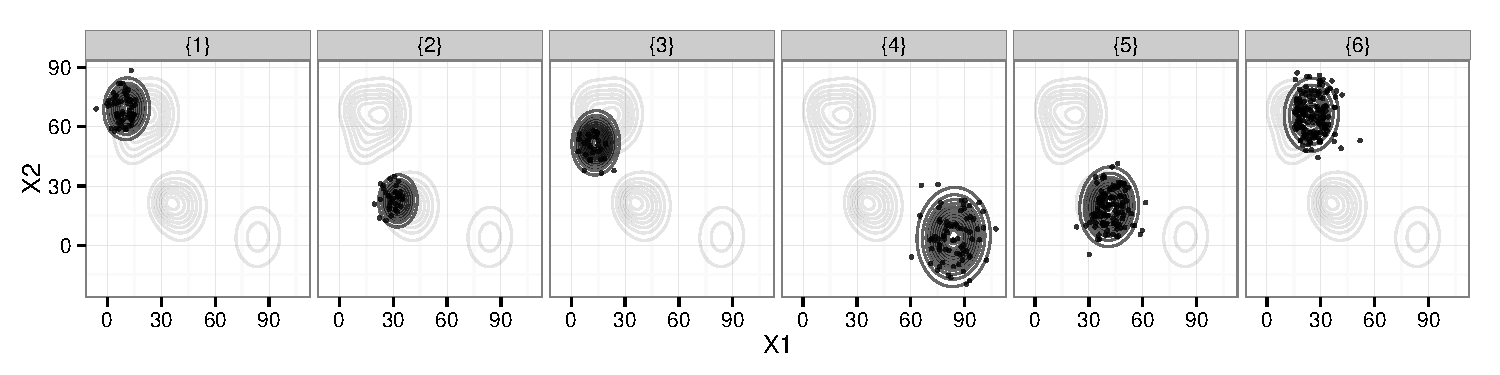
\includegraphics[trim=0cm 0cm 0cm 0cm,width=\textwidth]{partition-example-part6.pdf} \\
 \end{tabular}
 \caption{Classification obtained considering the component partition $\{ \{1\}, \{2\}, \{3\}, \{4\}, \{5\}, \{6\} \}$ with 6 parts in sample $X_{500}$.}\label{ex_part6}
\end{center}
\end{figure}

If we consider a different partition such as
\[\mathcal{I}_3 = \{\{1, 3, 6\},\{2, 5\},\{4\}\}\]
which is grouping those components with closest mean, we get the 3 clusters given in Figure~\ref{ex_part3a}. We have included the isodensity curves of pdf $\hat{f}_{\{1,3,6\}}$, $\hat{f}_{\{2, 5\}}$ and $\hat{f}_{\{4\}}$ given by

\[
%\left\{
\begin{array}{r c l}
\hat{f}_{\{1,3,6\}} & = & \frac{1}{0.52}(0.13 \phi(\;\cdot\; ; \hat{\m\mu}_1, \hat{\m\Sigma}_1) + 0.07 \phi(\;\cdot\; ; \hat{\m\mu}_3, \hat{\m\Sigma}_3) + 0.32 \phi(\;\cdot\; ; \hat{\m\mu}_6, \hat{\m\Sigma}_6)), \\
\hat{f}_{\{2, 5\}} & = &  \frac{1}{0.33}(0.09 \phi(\;\cdot\; ; \hat{\m\mu}_2, \hat{\m\Sigma}_2) + 0.24 \phi(\;\cdot\; ; \hat{\m\mu}_5, \hat{\m\Sigma}_5)), \\
\hat{f}_{\{4\}} & = &\phi(\;\cdot\; ; \hat{\m\mu}_4, \hat{\m\Sigma}_4).
\end{array}
%\right.
\]



\begin{figure}[!h]
\begin{center}
\begin{tabular}{cc}
  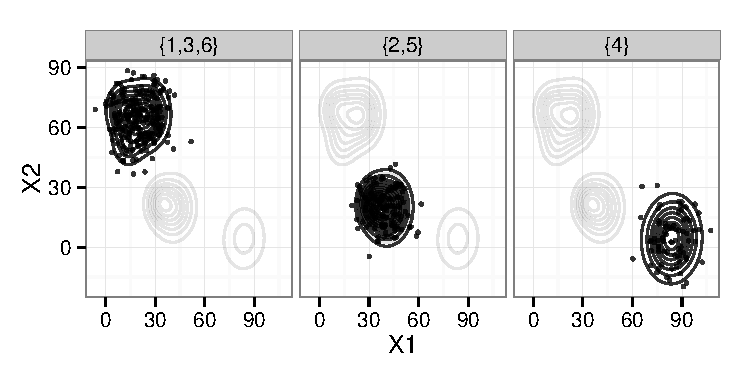
\includegraphics[trim=0cm 0cm 0cm 0cm,width=0.6\textwidth]{partition-example-part3a.pdf} \\
 \end{tabular}
 \caption{Classification obtained considering the component partition $\{\{1, 3, 6 \}, \{2, 5\}, \{5\}\}$ with 3 parts in sample $X_{500}$.}\label{ex_part3a}
\end{center}
\end{figure}

Consider now the hierarchical combination of components given by the following sequence of partitions
\begin{equation}
\begin{array}{r c c}
\mathcal{H}(\mathcal{I}) &=& \{ \{\{1\},\{2\},\{3\},\{4\},\{5\},\{6\}\}, \\
   & & \{\{1, 6\},\{2\},\{3\},\{4\},\{5\} \}, \\
   & &    \{\{1, 6, 3\},\{2\},\{4\},\{5\} \}, \\
   & &    \{\{1, 6, 3\},\{2, 5\},\{4 \} \}, \\
    & &   \{\{1, 6, 3\},\{2, 4, 5\} \}, \\
   & &    \{\{1, 2, 3, 4, 5, 6\}\} \}.
\end{array}
\label{hier_ex}
\end{equation}
Each partition from the hierarchical combination of components given by \ref{hier_ex} defines a clustering where each element is classified to one of the parts of each partition. Therefore, a hierarchical combination of components defines a hierarchical clustering structure. Figure~\ref{hierarchical} shows the hierarchical clustering obtained in sample $X_{500}$ using the hierarchical combination of components given in Eq~\ref{hier_ex}. The first partition $\{\{1\},\{2\},\{3\},\{4\},\{5\},\{6\}\}$ defines a clustering with 6 clusters, the partition $\{\{1, 6\}, \{3\},\{2\},\{4\},\{5\} \}$ defines a clustering with 5 clusters, and so on.

\begin{figure}[thbp]
\begin{center}
\begin{tabular}{cc}
  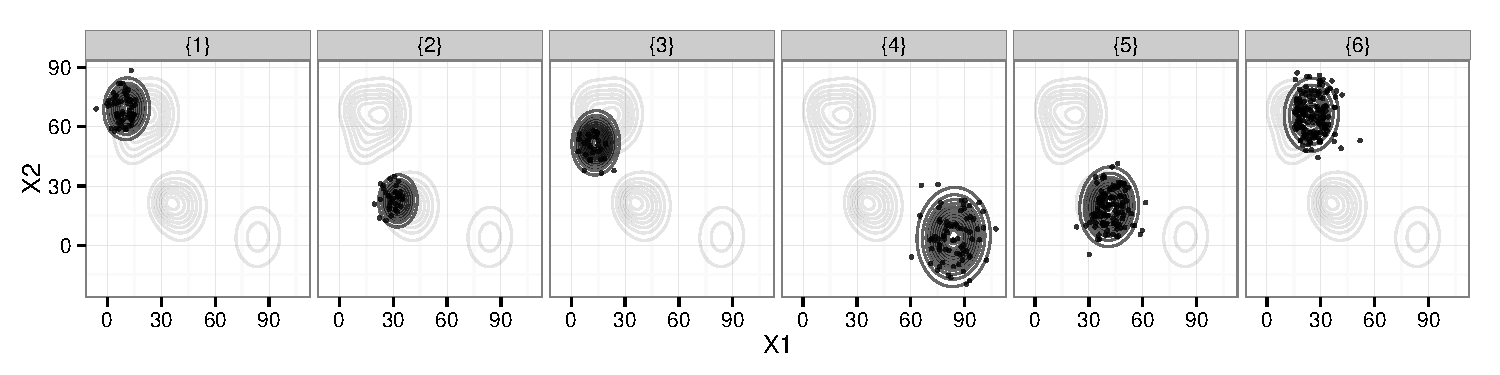
\includegraphics[trim=0cm 0cm 0cm 0cm,width=\textwidth]{partition-example-part6.pdf} \\
    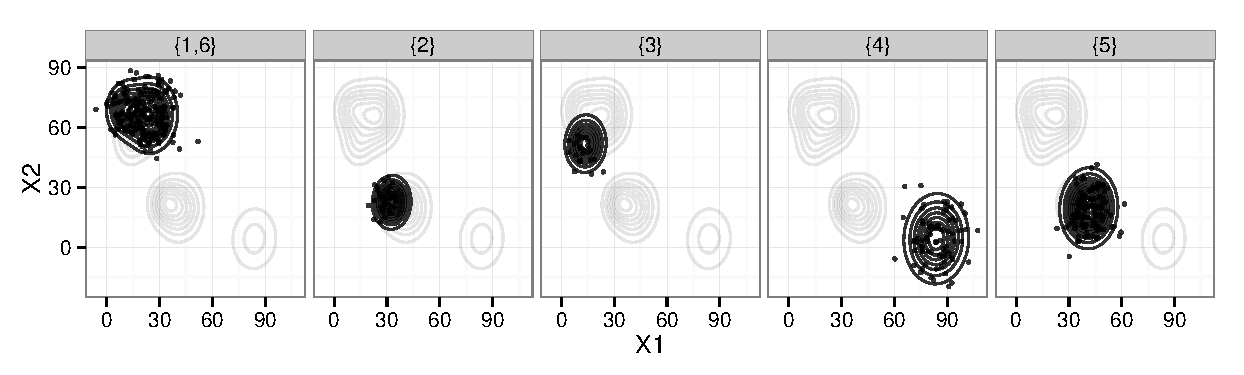
\includegraphics[trim=0cm 0cm 0cm 0cm,width=0.83\textwidth]{partition-example-part5.pdf} \\
      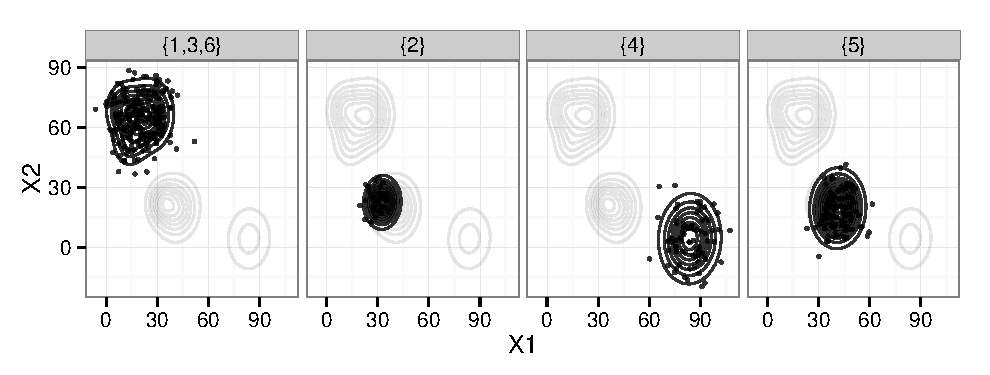
\includegraphics[trim=0cm 0cm 0cm 0cm,width=0.67\textwidth]{partition-example-part4.pdf} \\
        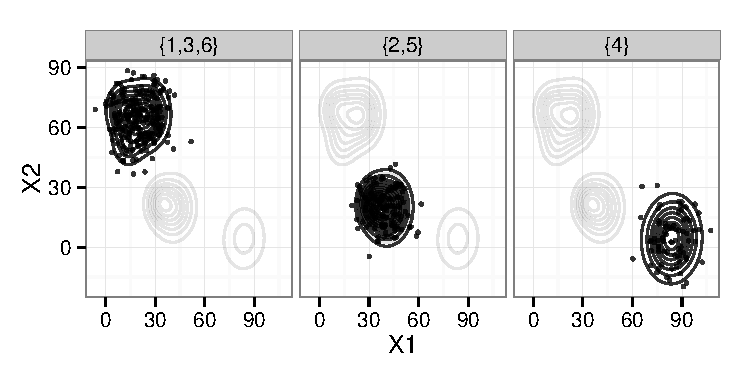
\includegraphics[trim=0cm 0cm 0cm 0cm,width=0.5\textwidth]{partition-example-part3a.pdf} \\
          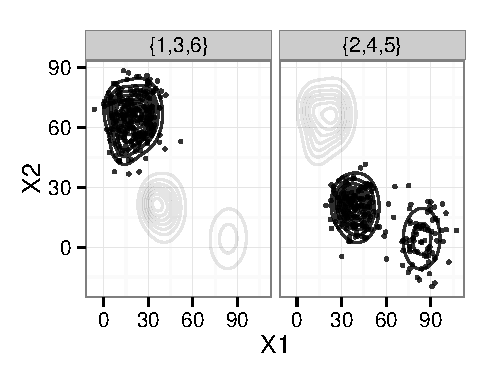
\includegraphics[trim=0cm 0cm 0cm 0cm,width=0.33\textwidth]{partition-example-part2.pdf} \\
            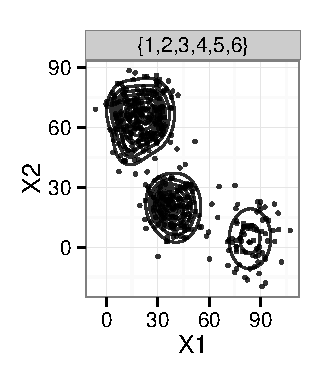
\includegraphics[trim=0cm 0cm 0cm 0cm,width=0.2\textwidth]{partition-example-part1.pdf}
 \end{tabular}
 \caption{Hierarchical cluster obtained by the hierarchical combination of components.}\label{hierarchical}
\end{center}
\end{figure}

In next section, for a given a finite mixture we review and propose different methods to decide how to merge its components only using information given by the posterior probabilities $\hat{\tau}_{i \mathcal{I}}$, $1\leq i \leq n$.

\section{Hierarchical approaches based on posterior probabilities}
\label{old_methods}

Once a finite mixture distribution is adjusted to a sample $X=\{x_1, \dots, x_n\}$, for any partition $\mathcal{I}_s = \{ I_1, \dots, I_s\}$ we can calculate the posterior probability vector  $\hat{\m\tau}_{i \mathcal{I}_s} = \left( \hat{\tau}_{i I_1} , \dots, \hat{\tau}_{i I_s}  \right)$ for each observation $x_i$, $1 \leq i \leq n$, of sample $X$. In this section we show different approaches to combine two parts $I_a$ and $I_b$ from a partition $\mathcal{I}_s$ into one part $I_a \cup I_b$, obtaining a new partition
\[
\mathcal{I}_{s, a \cup b} = \left( \mathcal{I}_s \setminus \{ I_a, I_b \} \right) \cup \left\{ \{ i | i \in I_a\cup I_b \} \right\}
\]
{\color{blue} la notaci\'{o} es complica!! cal??? suposo que necessites indicar les dues parts que ajuntes}
\[
\mathcal{I}_{s-1,a \cup b} = \left( \mathcal{I}_s \setminus \{ I_a, I_b \} \right) \cup \left\{ \in I_a\cup I_b \right\}
\]
with $s-1$ parts. $\mathcal{I}_{s-1,a \cup b}$ is formed with the parts available in $\mathcal{I}_{s}$ except $I_a$ and  $I_b$, and the new part $I_a \cup I_b$. Starting from partition $\{ \{1\}, \{2\}, \dots \{k\}\}$ and merging sequentially, each method in this section yields to an algorithm to build a hierarchical combination of components.

Let us remarks that all the methods presented in this article are based only on the information contained in the posterior probability vectors $\{ \hat{\m\tau}_{1 \mathcal{I}_s},\dots, \hat{\m\tau}_{n \mathcal{I}_s} \}$. {\color{blue} si es parla de la matriu de posterioris abans aqu\'{\i} es pot tornar a indicar.}


\subsection{Approach based on the total Entropy}

The Entropy of a posterior probability vector $\hat{\m\tau}_{i \mathcal{I}_s} = \left( \hat{\tau}_{i I_1} , \dots, \hat{\tau}_{i I_s}  \right)$ of an observation $x_i$, $1 \leq i \leq n$ is
\[
Ent( \hat{\m \tau}_{i \mathcal{I}_s} ) = \sum_{j=1}^s \hat{\tau}_{i I_j}  log(\hat{\tau}_{i I_j} ).
\]
$Ent( \hat{\m \tau}_{i \mathcal{I}_s} )$ is a convex function with its minimum at $(\frac{1}{s},\dots,\frac{1}{s})$. In terms of posterior probabilities, the minimum is obtained when the probability of $x_i$ being generated by each distributions with pdf $\hat{f}_{I_1}, \dots, \hat{f}_{I_s}$ is the same conditioned to $x_i$ being generated by the mixture distribution given by Eq.~\ref{mixt_part}.

Due to the fact the previous minimum is the point with more ``confusion'' between parts, \cite{baudry2010combining} proposed to merge those components, $I_a$ and $I_b$, such that $\sum_{i=1}^n Ent( \hat{\m \tau}_{i \mathcal{I}_{s-1, a \cup b}} )$ is minimum. In other words, their criteria proposes to merge those components that after merging, the sum of the entropy of the resulting posterior probability vectors is minimum.

The calculation of the previous criteria depends on the posterior probability of each part $\hat{\tau}_{iI_1}, \dots,\hat{\tau}_{iI_s}$. To reduce calculations \cite{baudry2010combining} proposed to combine those parts, $I_a$ and $I_b$, such that the difference
\begin{multline*}
\Delta Ent_{const}(\hat{\m \tau}_{i \mathcal{I}_s}, a, b) = \sum_{i=1}^n Ent( \hat{\m \tau}_{i \mathcal{I}_{s-1, a \cup b}}) - \sum_{i=1}^n Ent( \hat{\m \tau}_{i \mathcal{I}_s}) =  \\ = \sum_{i=1}^n  \left( \hat{\tau}_{i I_{a\cup b}}  log(\hat{\tau}_{i I_{a\cup b}} ) +  \sum_{\substack{j=1 \\
                                                            j \neq a, b}}^s \hat{\tau}_{i I_j}  log(\hat{\tau}_{i I_j} ) \right)  - \sum_{i=1}^n \sum_{j=1}^s \hat{\tau}_{i I_j}  log(\hat{\tau}_{i I_j} ) = \\  =   \sum_{i=1}^n  (\hat{\tau}_{iI_a}+\hat{\tau}_{iI_b}) \log(\hat{\tau}_{iI_a} + \hat{\tau}_{iI_b}) - \sum_{i=1}^n \left\{ \hat{\tau}_{iI_a} \log(\hat{\tau}_{iI_a}) + \hat{\tau}_{iI_b} \log(\hat{\tau}_{iI_b})\right\}
\end{multline*}
is maximum. Doing so, the criteria depends only on the posterior probability of $\hat{\tau}_{iI_a}$ and $\hat{\tau}_{iI_b}$. {\color{blue} Afegir qu\`{e} significa aix\`{o}, \'{e}s a dir, aqu\'{\i} es conclouque aquest m\`{e}tode nom\'{e}s dep\`{e}s de dues columnes de la matriu de posterioris, i aix\`{o} perqu\`{e} era important.}

{\color{blue} Marc, a mi em lia molt tota la notaci\'{o}, jo trobo a faltar explicar la idea intu\"{\i}tiva que hi ha aqu\'{\i} al darrera (pq entropia,...). Potser \'{e}s una tonteria per\`{o} no caldria parlar tamb\'{e} de la simetria dels m\`{e}todes? no v\`{a}rem quedar que era una q\"{u}esti\'{o} important que els diferenciava??}

\subsection{Directed Estimated misclassification Probabilities (DEMP) approach}

A different approach is introduced in \cite{hennig2010methods}. Hennig proposed to combine the two parts $I_a$ and $I_b$ from $ \mathcal{I}_s$ such that \emph{the probability of classifying an observation generated from component $\hat{f}_{I_a}$ to component $\hat{f}_{I_b}$} is maximum.

To estimate that probability,  \cite{hennig2010methods} suggested to use a consistent estimator, the Directed Estimated misclassification Probabilities (DEMP). Using the notation previously introduced, the estimator is written as
\[
\frac{ \frac{1}{n} \sum_{i=1}^n {\hat{\tau}_{iI_a} \mathbbm{1}\left( \forall j\; \hat{\tau}_{i I_{b}} \geq \hat{\tau}_{iI_j} \right)}}{ \hat{\pi}_{I_a}},
\]
where $\mathbbm{1}\left( \cdot \right)$ is the indicator function. Moreover, because $ \hat{\pi}_{I_a} = \frac{1}{n} \sum_{i=1}^n \hat{\tau}_{iI_a}$, the estimator can be rewritten in terms of the posterior probability vector as
\begin{equation}\label{demp_criteria}
DEMP_{prop}(\hat{\m \tau}_{i \mathcal{I}_s}, a, b) =\frac{ \sum_{i=1}^n {\hat{\tau}_{iI_a} \mathbbm{1}\left( \forall j\; \hat{\tau}_{i I_{b}} \geq \hat{\tau}_{iI_j} \right)}}{\sum_{i=1}^n \hat{\tau}_{iI_a} }.
\end{equation}

Then, Henning proposed to combine parts $I_a$ and $I_b$, such that the $DEMP_{prop}(\hat{\m \tau}_{i \mathcal{I}_s}, a, b)$ is maximum. {\color{blue} \'{E}s correcte aix\`{o} que he afegit?} 

Nota that the idea behind the approach proposed by Baudry \emph{et al.} is different from the one proposed by Hennig. For the former, the confusion between part $a$ and part $b$ is measured by measuring how different $\hat{\m \tau}_{i \mathcal{I}_a}$ and $\hat{\m \tau}_{i \mathcal{I}_b}$ are, for all $i$, $1\leq i \leq n$, independently. In contrast, Hennig measures the confusion between part $a$ and part $b$ by counting the number of times an observation is classified to $b$, weighing the counting with respect the posterior probability of begin generated by $\hat{f}_{I_a}$ (see Eq.~\ref{demp_criteria}).

For an observation generated from a pdf $\hat{f}_{I_a}$, the role played by the indicator function in Equation~\ref{demp_criteria} is to count the number of times the observation is classified to part $I_b$, this counting is used to estimate the probability of classifying an observation to part $I_b$. A different approach can be considered if instead of using the probability of classifying to part $b$, the probability of being generated by part $b$ is used.

{\color{blue} Aquí posaria un nou apartat 3.3 DEGP, per deixar clar que tu proposes un nou m\`{e}tode utilitzant la idea de'n Henning juntament amb la de Longford i Bartosova.}

\cite{longford2014} proposed to estimate the probability that an observation is generated by component $\hat{f}_{I_b}$ conditioned to the fact that the observation has been generated by either $\hat{f}_{I_a}$ or $\hat{f}_{I_b}$. In this case, the indicator function in Equation~\ref{demp_criteria} takes the form $\frac{\hat{\tau}_{iI_b}}{\hat{\tau}_{iI_a} + \hat{\tau}_{iI_b}}$. The main difference between these approaches is that while $\mathbbm{1}\left( \forall j\; \hat{\tau}_{i I_{b}} \geq \hat{\tau}_{iI_j} \right)$ estimates the probability of classifying an observation $x_i$ to $I_b$, $\frac{\hat{\tau}_{iI_b}}{\hat{\tau}_{iI_a} + \hat{\tau}_{iI_b}}$ estimates the probability of $x_i$ being generated by $\hat{f}_{I_b}$ conditioned to $x_i$  being generated by $\hat{f}_{I_a}$ or $\hat{f}_{I_b}$.

In \cite{longford2014} the estimator they proposed was obtained by simulating a large amount of observation from component $\hat{f}_{I_a}$. Here, we use the idea introduced by \cite{longford2014} and the weighing approach used in DEMP estimator, to build a similar but new estimator,

\begin{equation}\label{demp2_criteria}
DEGP_{prop}(\hat{\m \tau}_{i \mathcal{I}_s}, a, b) =\frac{ \sum_{i=1}^n \hat{\tau}_{iI_a} \hat{\tau}_{iI_b}(\hat{\tau}_{iI_a} + \hat{\tau}_{iI_b})^{-1}  }{\sum_{i=1}^n \hat{\tau}_{iI_a} }.
\end{equation}
Then we combine parts $I_a$ and $I_b$, such that the $DEGP_{prop}(\hat{\m \tau}_{i \mathcal{I}_s}, a, b)$ is maximum. {\color{blue} \'{E}s correcte aix\`{o} que he afegit?} By similarity to DEMP estimator, from now on we referer it as the Directed Estimated generation Probabilities estimator (DEGP). The main difference between DEGP estimator and the one proposed by Longford and Bartosova is that the former is obtained from sample $X$, the later is obtained from simulation once the parameters of mixture $f$ have been obtained.


\subsection{The log-ratio approaches}
\label{lr_approach}

In the total Entropy approach, the idea of confusion between components is build over the idea that the closer the posterior probability vector are from $(\frac{1}{s}, \dots, \frac{1}{s})$ the more confused are the components. In contrast, in DEMP and DEGP approaches the idea of confusion is build over the probability of classifying an observation to one component when the observation was generated from another component.

Using this two ideas, we present two different families of methods which build the idea of confusion between part $I_a$ and $I_b$ by comparing the components $\hat{\tau}_{iI_a}$ and $\hat{\tau}_{iI_b}$ relatively inside the posterior probability vector $\hat{\m \tau}_{i \mathcal{I}_s}$.

The first family of approaches we propose measure the chances of confusing $I_b$ with $I_a$. The idea is that if an observation was generated from the probability density function $\hat{f}_{I_a}$, the higher is $\hat{\tau}_{iI_b}$ respect to $\hat{\tau}_{iI_a}$ the higher are the chances of confusing $I_b$ with $I_a$. To measure the relative differences between  $\hat{\tau}_{iI_b}$ and $\hat{\tau}_{iI_a}$, we propose to use the log ratio between them, i.e $log( \hat{\tau}_{iI_b}/\hat{\tau}_{iI_a})$.

The second family of approaches we propose, measure the chances of confusing $I_b$ with $I_a$  by measuring how different are $(\frac{\hat{\tau}_{iI_a}}{\hat{\tau}_{iI_a} + \hat{\tau}_{iI_b}}, \frac{\hat{\tau}_{iI_b}}{\hat{\tau}_{iI_a} + \hat{\tau}_{iI_b}})$ from $(\frac{1}{2}, \frac{1}{2})$. {\color{blue} Perqu\`{e}? justifica-ho millor.}To measure the difference between these two posterior probability vectors, we use the norm defined in the Simplex space. The norm of a posterior probability vector, $\| (\hat{\tau}_{iI_a}, \hat{\tau}_{iI_b}) \|$  as defined in \cite{aitchison2002simplicial} is
\[
\left\| (\hat{\tau}_{iI_a}, \hat{\tau}_{iI_b}) \right\| = \log \left(\frac{ \hat{\tau}_{iI_b} }{ \hat{\tau}_{iI_a} }\right)^2.
\]
The norm $\| (\hat{\tau}_{iI_a}, \hat{\tau}_{iI_b}) \|$ measures how far is the posterior probability vector $(\hat{\tau}_{iI_a}, \hat{\tau}_{iI_b})$ of the posterior probability vector $(\frac{1}{2}, \frac{1}{2})$.

Using this two measures we can build two approaches: the first one measures how likely is to incorporate part $b$ into part $a$. To do so, we propose to combine those parts $I_a$ and $I_b$ maximising the criteria
\[
LOG_{const}( \hat{\m \tau}_{i \mathcal{I}_s}, a, b) = \sum_{i=1}^n \log \left(\frac{ \hat{\tau}_{iI_b} }{ \hat{\tau}_{iI_a} }\right).
\]
The second approach measures how far are $(\frac{\hat{\tau}_{iI_a}}{\hat{\tau}_{iI_a} + \hat{\tau}_{iI_b}}, \frac{\hat{\tau}_{iI_b}}{\hat{\tau}_{iI_a} + \hat{\tau}_{iI_b}})$ from $(\frac{1}{2}, \frac{1}{2})$. To do so, we propose to combine those parts $I_a$ and $I_b$ maximising the criteria
\[
LOG^2_{const}( \hat{\m \tau}_{i \mathcal{I}_s}, a, b) = -\sum_{i=1}^n \log \left(\frac{ \hat{\tau}_{iI_b} }{ \hat{\tau}_{iI_a} }\right)^2.
\]

%%% prop approach
This two approaches average the scores obtained for each observation $x_i$ from $X$. If instead of this, we weight the scores respect to $ \hat{\tau}_{iI_a}$  as in DEMP approach, we get two new approaches. The first combines those parts $I_a$ and $I_b$ maximising the criteria
\[
LOG_{prop}( \hat{\m \tau}_{i \mathcal{I}_s}, a, b) = \frac{ \sum_{i=1}^n \hat{\tau}_{iI_a} \log \left(\frac{ \hat{\tau}_{iI_b} }{ \hat{\tau}_{iI_a} }\right)}{\sum_{i=1}^n\hat{\tau}_{iI_a}}.
\]
The second, combines those parts $I_a$ and $I_b$ maximising the criteria
\[
LOG^2_{prop}( \hat{\m \tau}_{i \mathcal{I}_s}, a, b) = \frac{ \sum_{i=1}^n \hat{\tau}_{iI_a} \left(-\log \left(\frac{ \hat{\tau}_{iI_b} }{ \hat{\tau}_{iI_a} }\right)^2\right)}{\sum_{i=1}^n\hat{\tau}_{iI_a}}.
\]


%%%%% dichotomic
A different approach can be obtained if instead of weighting the scores respect $ \hat{\tau}_{iI_a}$ we only consider the score for those observation $x_i$ which are classified to part $I_a$, i.e. $x_i$ for which $\forall j\; \hat{\tau}_{i I_{a}} \geq \hat{\tau}_{iI_j}$ holds. This dichotomic approach (each observation is either classified to part $I_a$ or to another part) allows us to introduce two different approaches: the first combines those parts $I_a$ and $I_b$ maximising the criteria
\[
LOG_{dich}( \hat{\m \tau}_{i \mathcal{I}_s}, a, b) = \frac{ \sum_{i=1}^n  \mathbbm{1}\left( \forall j\; \hat{\tau}_{i I_{a}} \geq \hat{\tau}_{iI_j} \right) \log \left(\frac{ \hat{\tau}_{iI_b} }{ \hat{\tau}_{iI_a} }\right)}{\sum_{i=1}^n \mathbbm{1}\left( \forall j\; \hat{\tau}_{i I_{a}} \geq \hat{\tau}_{iI_j} \right)}.
\]
The second combines those parts $I_a$ and $I_b$ maximising the criteria
\[
LOG^2_{dich}( \hat{\m \tau}_{i \mathcal{I}_s}, a, b) = \frac{ \sum_{i=1}^n \mathbbm{1}\left( \forall j\; \hat{\tau}_{i I_{a}} \geq \hat{\tau}_{iI_j} \right) \left(-\log \left(\frac{ \hat{\tau}_{iI_b} }{ \hat{\tau}_{iI_a} }\right)^2\right)}{\sum_{i=1}^n \mathbbm{1}\left( \forall j\; \hat{\tau}_{i I_{a}} \geq \hat{\tau}_{iI_j} \right)}.
\]

To summarise, using log-ratio approaches we have build two different criteria for measuring the confusion between two parts $(\log ( \hat{\tau}_{iI_b} / \hat{\tau}_{iI_a} $ and $-\log (\hat{\tau}_{iI_b} / \hat{\tau}_{iI_a} )^2)$. For each of them, we have introduce three different strategies to combine the scores obtained for each observation $x_i$. This three strategies are
\begin{description}
\item[const] for each observation, we calculate the confusion measure and we sum (or average) all the confusion measurements.
\item[prop] for each observation, we calculate the confusion measure and we calculate a weighted mean of them according to the probability of an observation to be generated from component $a$.
\item[dich] for each observation, we calculate the confusion measure and we average the confusions only on those observations associated to component $a$.
\end{description}




\section{Unifying the approaches}
\label{confusion}

Let $\lambda(\hat{\m \tau}_{i \mathcal{I}_s}, a, b)$ be a function measuring the chances of mixing up the mixture component $\hat{f}_{I_a}$ by the mixture component $\hat{f}_{I_b}$ when $\hat{\m \tau}_{i \mathcal{I}_s}$ is known, i.e. selecting $\hat{f}_{I_b}$ when one have to select $\hat{f}_{I_a}$. In Section~\ref{old_methods} we have seen different alternatives to measure such confusion. This alternatives were

\begin{itemize}
\item the entropy presented by Baudry \emph{et al.},
\[\lambda(\hat{\m \tau}_{i \mathcal{I}_s}, a, b) = (\hat{\tau}_{iI_a}+\hat{\tau}_{iI_b}) \log(\hat{\tau}_{iI_a} + \hat{\tau}_{iI_b}) - \hat{\tau}_{iI_a} \log(\hat{\tau}_{iI_a}) + \hat{\tau}_{iI_b} \log(\hat{\tau}_{iI_b}),\]
\item the misclassification probability presented by Hennig, \[\lambda(\hat{\m \tau}_{i \mathcal{I}_s}, a, b) = \mathbbm{1}\left( \forall j\; \hat{\tau}_{i I_{b}} \geq \hat{\tau}_{iI_j} \right),\]
\item the ``misgeneration'' probability presented by Longford and Bartosova, \[\lambda(\hat{\m \tau}_{i \mathcal{I}_s}, a, b) = \frac{\hat{\tau}_{iI_b}}{\hat{\tau}_{iI_a} + \hat{\tau}_{iI_b}},\]
\item the Aitchison norm, \[\lambda(\hat{\m \tau}_{i \mathcal{I}_s}, a, b) = \log (\frac{ \hat{\tau}_{iI_b} }{ \hat{\tau}_{iI_a} })^2 \text{ and}\]
\item the log-ratio \[ \lambda(\hat{\m \tau}_{i \mathcal{I}_s}, a, b) = \log (\frac{ \hat{\tau}_{iI_b} }{ \hat{\tau}_{iI_a} }).\]
\end{itemize}

All this approaches provides us with different ways to measure the confusion between different components. Moreover, all of them are based only on the posterior probability
vector $(\hat{\tau}_{i I_{1}}, \dots, \hat{\tau}_{i I_{s}})$.

Let $\omega(\hat{\m \tau}_{i \mathcal{I}_s}, a)$ be a function measuring the relevance $\hat{\m \tau}_{i \mathcal{I}_s}$ to measure the chances of mixing up  the mixture component $\hat{f}_{I_a}$. In Subsection~\ref{lr_approach} we have seen three different criteria:

\begin{itemize}
\item each observation is equally relevant to measure the chances of mixing up  $\hat{f}_{I_a}$,
\[\omega(\hat{\m \tau}_{i \mathcal{I}_s}, a) = const,\]
\item the relevance is equal to the posterior probability of being generated by  $\hat{f}_{I_a}$,
\[\omega(\hat{\m \tau}_{i \mathcal{I}_s}, a) =  \hat{\tau}_{iI_a} \text{ and}\]
\item  only the posterior probability of observations classified to part   $I_a$ are relevant
\[\omega(\hat{\m \tau}_{i \mathcal{I}_s}, a) = \mathbbm{1}\left( \forall j\; \hat{\tau}_{i I_{a}} \geq \hat{\tau}_{iI_j} \right).\]
\end{itemize}


\begin{table}
\begin{tabular}{c  c | >{\centering}m{0.7in} | >{\centering}m{0.8in} | >{\centering}m{0.7in} | m{0in}}
 & \multicolumn{1}{c}{} & \multicolumn{3}{c}{$\omega(\boldsymbol\tau_i, a)$} &\\

 & \multicolumn{1}{c}{} & \multicolumn{1}{c}{} & \multicolumn{1}{c}{} & \multicolumn{1}{c}{} & \multicolumn{1}{c}{}\\

 & \multicolumn{1}{c}{} & \multicolumn{1}{c}{1} & \multicolumn{1}{c}{$\tau_{ia}$} & \multicolumn{1}{c}{$\mathlarger{\mathbbm{1}}\left\{ \forall \ell\;\tau_{ia}\geq \tau_{i\ell}  \right\}$} &\\ \cline{3-5}

& $\large\substack{(\tau_{i a}+\tau_{i b}) \log(\tau_{i a} + \tau_{i b}) - \\ - \tau_{i a} \log(\tau_{i a}) - \tau_{i b} \log(\tau_{i b}) }$ & {\small const-entr}\\($\Delta Ent_{const}$)& {\small prop-entr} & {\small dich-entr } &\\[5em] \cline{3-5}

& $\mathlarger{\mathbbm{1}}\left\{  \forall \ell \; \tau_{hb} \geq \tau_{h\ell}  \right\}$ & {\small const-demp} & {\small prop-demp}\\($DEMP_{prop}$)  & {\small dich-demp} & \\[5em] \cline{3-5}

\rotatebox[origin=c]{90}{$\lambda(\boldsymbol\tau_i, a, b)$}& ${\tau_{i b}}({\tau_{i a}+\tau_{i b}})^{-1}$ & {\small const-degp} &  {\small prop-degp}\\($DEGP_{prop}$) & {\small dich-degp} &\\[5em] \cline{3-5}

& $\log{\tau_{i b} / \tau_{i a}}$ & {\small const-log}\\($LOG_{const}$) & {\small prop-log}\\($LOG_{prop}$) & {\small dich-log}\\($LOG_{dich}$) &\\[5em] \cline{3-5}

& $(\log{\tau_{i b} / \tau_{i a}})^2$ & {\small const-norm}\\($LOG^2_{const}$) & {\small prop-norm}\\($LOG^2_{prop}$) & {\small dich-norm}\\($LOG^2_{dich}$)  &\\[5em] \cline{3-5}
\end{tabular}
\caption{Different combinations of score functions}
\label{table_methods}
\end{table}

For a partition $\mathcal{I}_s = \{ I_1, \dots, I_s\}$ and with  functions $\lambda(\hat{\m \tau}_{i \mathcal{I}_s}, a, b)$ and $\omega(\hat{\m \tau}_{i \mathcal{I}_s}, a)$ fixed, we can define a mixture component merging approach as follows: if $\hat{\m\tau}_{i \mathcal{I}_s} = \left( \hat{\tau}_{i I_1} , \dots, \hat{\tau}_{i I_s}  \right)$ are the posterior probability vectors of observation $x_i$, $1 \leq i \leq n$,  merge those two parts $I_a$ and $I_b$, into one part $I_a \cup I_b$ which maximise
\begin{equation}\label{unifying_equation}
S_{\omega, \lambda}( \hat{\m \tau}_{i \mathcal{I}_s}, a, b) = \frac{\sum_{i=1}^n \omega(\hat{\tau}_{i \mathcal{I}_s}, I_a) \lambda(\hat{\tau}_{i \mathcal{I}_s}, I_a, I_b)}{\sum_{i=1}^n \omega(\hat{\tau}_{i \mathcal{I}_s}, I_a) }.
\end{equation}


The general confusion measure given by Equation~\ref{unifying_equation} contains all the approaches introduced in Section~\ref{old_methods}. Note that when $\omega(\hat{\tau}_{i \mathcal{I}_s}, I_a) = const$ maximising Equation~\ref{unifying_equation} is equivalent to maximise
\[
S_{\omega, \lambda}( \hat{\m \tau}_{i \mathcal{I}_s}, a, b) = \sum_{i=1}^n \lambda(\hat{\tau}_{i \mathcal{I}_s}, I_a, I_b)
\]
and therefore, Equation~\ref{unifying_equation} also includes as particular cases the Entropy approach, $LOG_{const}$ and $LOG^2_{const}$ approaches. Moreover, it permits to introduce a broad range of new approaches by varying functions $\lambda(\hat{\m \tau}_{i \mathcal{I}_s}, a, b)$ and $\omega(\hat{\m \tau}_{i \mathcal{I}_s}, a)$. Particularly, by using th functions $\lambda(\hat{\m \tau}_{i \mathcal{I}_s}, a, b)$ and $\omega(\hat{\m \tau}_{i \mathcal{I}_s}, a)$ already defined in Section~\ref{old_methods} we have all the combinations given by Table~\ref{table_methods}. Note that the method with $\lambda(\hat{\m \tau}_{i \mathcal{I}_s}, a, b) =  \mathlarger{\mathbbm{1}}\left\{  \forall \ell \; \tau_{hb} \geq \tau_{h\ell}  \right\}$ and  $\omega(\hat{\m \tau}_{i \mathcal{I}_s}, a) = \mathlarger{\mathbbm{1}}\left\{  \forall \ell\; \; \tau_{ia} \geq \tau_{i\ell}  \right\}$ it always evaluate 0, and therefore, it is of no use.

In the following section we compare the methods proposed in Table~\ref{table_methods} in different scenarios.

\section{Comparing the methods}
\label{comparison}

Consider the finite mixture
\begin{equation}\label{two_mixture}
f_2 = \pi_a \hat{f}_{I_a} + (1 - \pi_a) \hat{f}_{I_b, \mu_b}
\end{equation}
with \emph{two} components, where component $\hat{f}_{I_a} = N(0, 1)$ is the univariate normal distribution with mean equal to $0$ and variance $1$, and component $\hat{f}_{I_b, \mu_b} = N(\mu_b, 1)$ is a normal distribution with mean $\mu_b$ and variance $1$, and the two mixture proportions are parameterised by $\pi_a$.

We have generated $m=100\;000$ different samples of size $n=500$ randomly generated from mixture $f_2$. We have evaluated each of the approaches proposed in Table~\ref{table_methods} by varying parameter $\pi_a$ between values $0.1, 0.2, \dots, 0.9$ and parameter $\mu_b$ varying between $0$ and $3$. For each approach and parameter value, we have calculated the mean of the scores obtained in the $m$ samples. In Figure~\ref{fig:mu_varying} the obtained means are represented. {\color{blue} a l'eix de les y'd de la figura 5 i 6 hauria d'indicar que \'{e}s la mitjana dels scores, a la caption tamb\'{e}. En general trobo que cal explicar millor qu\`{e} representes i qu\`{e} esperaries obtenir. No vols dir que la paraula score la fas servir per coses diferents? Una altra cosa de notaci\'{o} per unificar, a la secci\'{o} 5.1 parles de each method $\mathcal{M}$ from Table~\ref{table_methods}.}

\begin{figure}[!t]
\centering
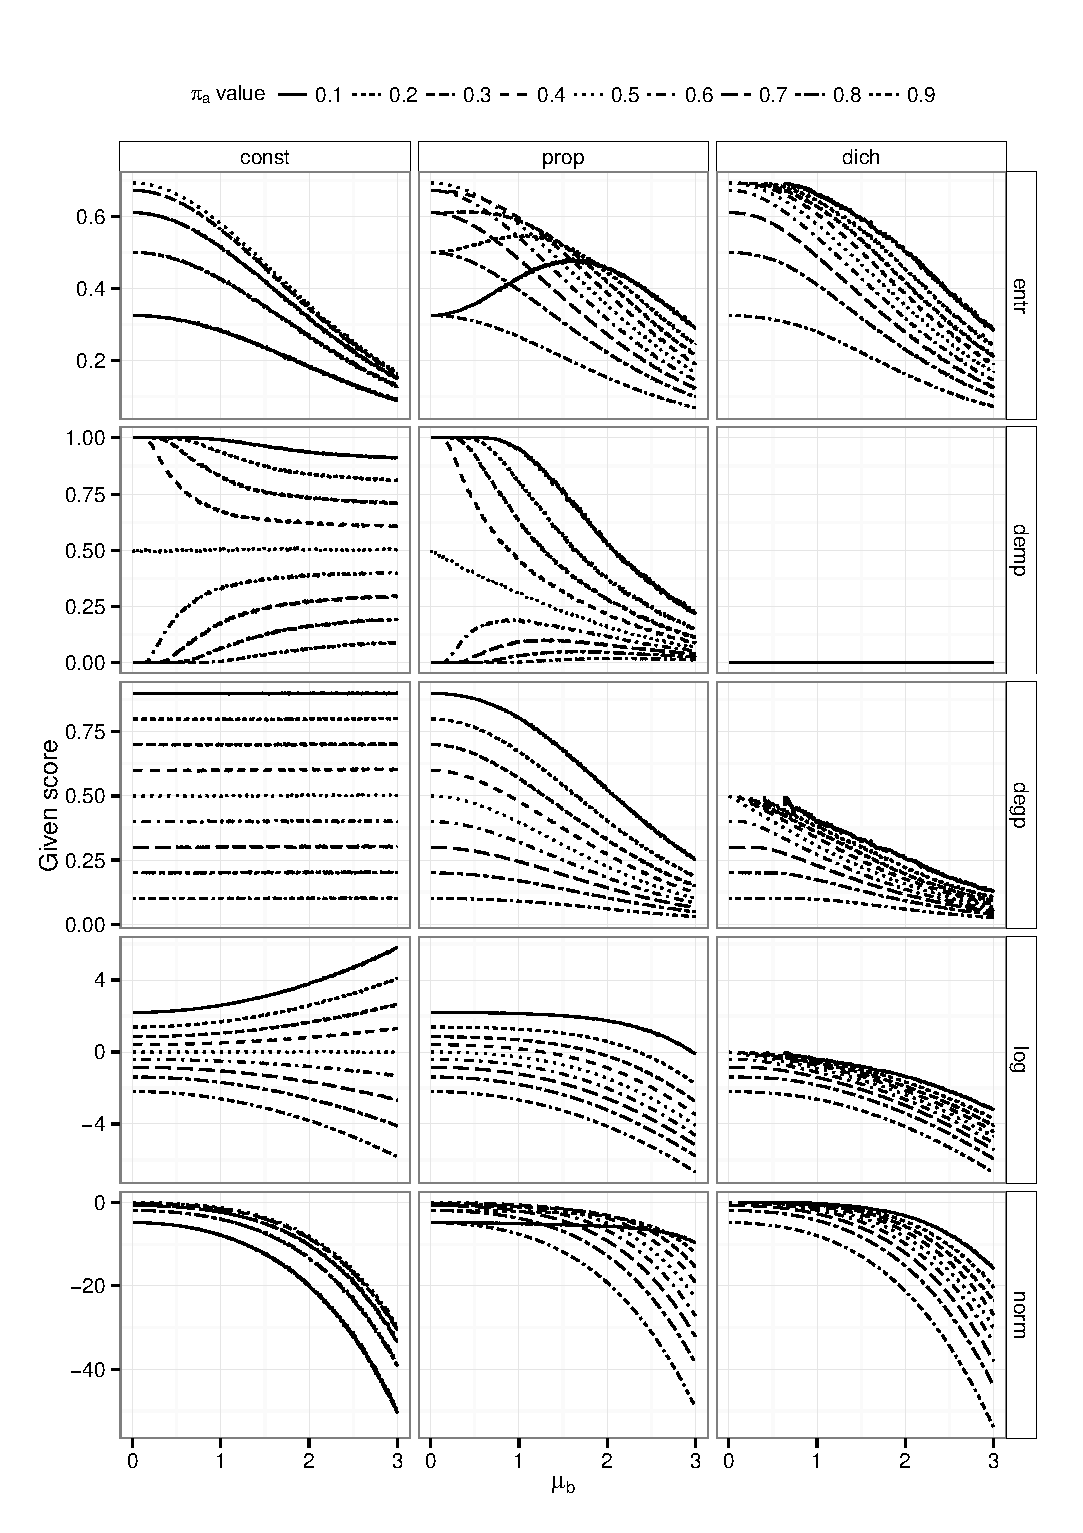
\includegraphics[scale=.5]{fig01all.eps}
\caption{Score calculated for methods described for different approaches of $\lambda$ and $\omega$ score when $\mu_b$ varying}
\label{fig:mu_varying}
\end{figure}

In the first column we have plot the methods for different proposed functions $\lambda$ using the function $\omega(\hat{\m \tau}_{i \mathcal{I}_s}, a) = 1$. In this scenario, only the entropy approach and the norm approach perform as expected, that is, the score decreases as the distance between the centre of distribution $\hat{f}_{I_a}$ and $\hat{f}_{I_b, \mu_b}$ increase. Moreover, for this two methods the obtained score the same when $\pi_a = 1- \pi_a$ {\color{blue} i per tant que les gr\`{a}fiques es solapen}.

In the second column we have plot the methods using the function $\omega(\hat{\m \tau}_{i \mathcal{I}_s}, a) = \hat{\tau}_{iI_a}$. In this case, all the methods perform as expected, the score decreases when $\mu_b$ increases. Note that the entropy and the norm methods become both again symmetric with respect to $\pi_a$ for values of $\mu_b$ close $0$.

In the third column, the score is represented using the function $\omega(\hat{\m \tau}_{i \mathcal{I}_s}, a) = \mathbbm{1}\left( \forall j\; \hat{\tau}_{i I_{a}} \geq \hat{\tau}_{iI_j} \right)$. In this case, all the approaches perform as expected except when $\lambda(\hat{\m \tau}_{i \mathcal{I}_s}, a, b) = \mathbbm{1}\left( \forall j\; \hat{\tau}_{i I_{b}} \geq \hat{\tau}_{iI_j} \right)$. In this case the function is constantly $0$, and therefore it is of no use to decide which components needs to be merged.


To compare, now we include another component keeping the two previous components inside the mixture. Consider the finite mixture
\begin{equation}\label{three_mixture}
f_3 = \pi_a \hat{f}_{I_a} + (0.5 - \pi_a) \hat{f}_{I_b, \mu_b} + 0.5 \hat{f}_{I_c}
\end{equation}
with three components. Component $\hat{f}_{I_a} = N(0, 1)$ is the normal with mean equal to $0$ and variance $1$, component $\hat{f}_{I_b, \mu_b} = N(\mu_b, 1)$ is a normal with mean $\mu_b$ and component $\hat{f}_{I_c} = N(3, 1)$ is the normal with mean equal to $3$ and variance $1$. The two first mixture proportions are parameterised by $\pi_a$ whereas the third one is constantly $0.5$.

Similar to the previous simulation, we have  randomly generated $m=100\;000$ different samples of size $n=500$ from mixture $f_3$. We have evaluated each approach proposed in Table~\ref{table_methods} by varying parameter $\pi_a$ between values $0.05, 0.1, \dots, 0.45$ and parameter $\mu_b$ varying between $0$ and $3$. For each approach and parameter value, we have calculated the mean of the score obtained in each of the $m$ samples. In Figure~\ref{fig:mu_varying3} the obtained means are represented.

\begin{figure}[!t]
\centering
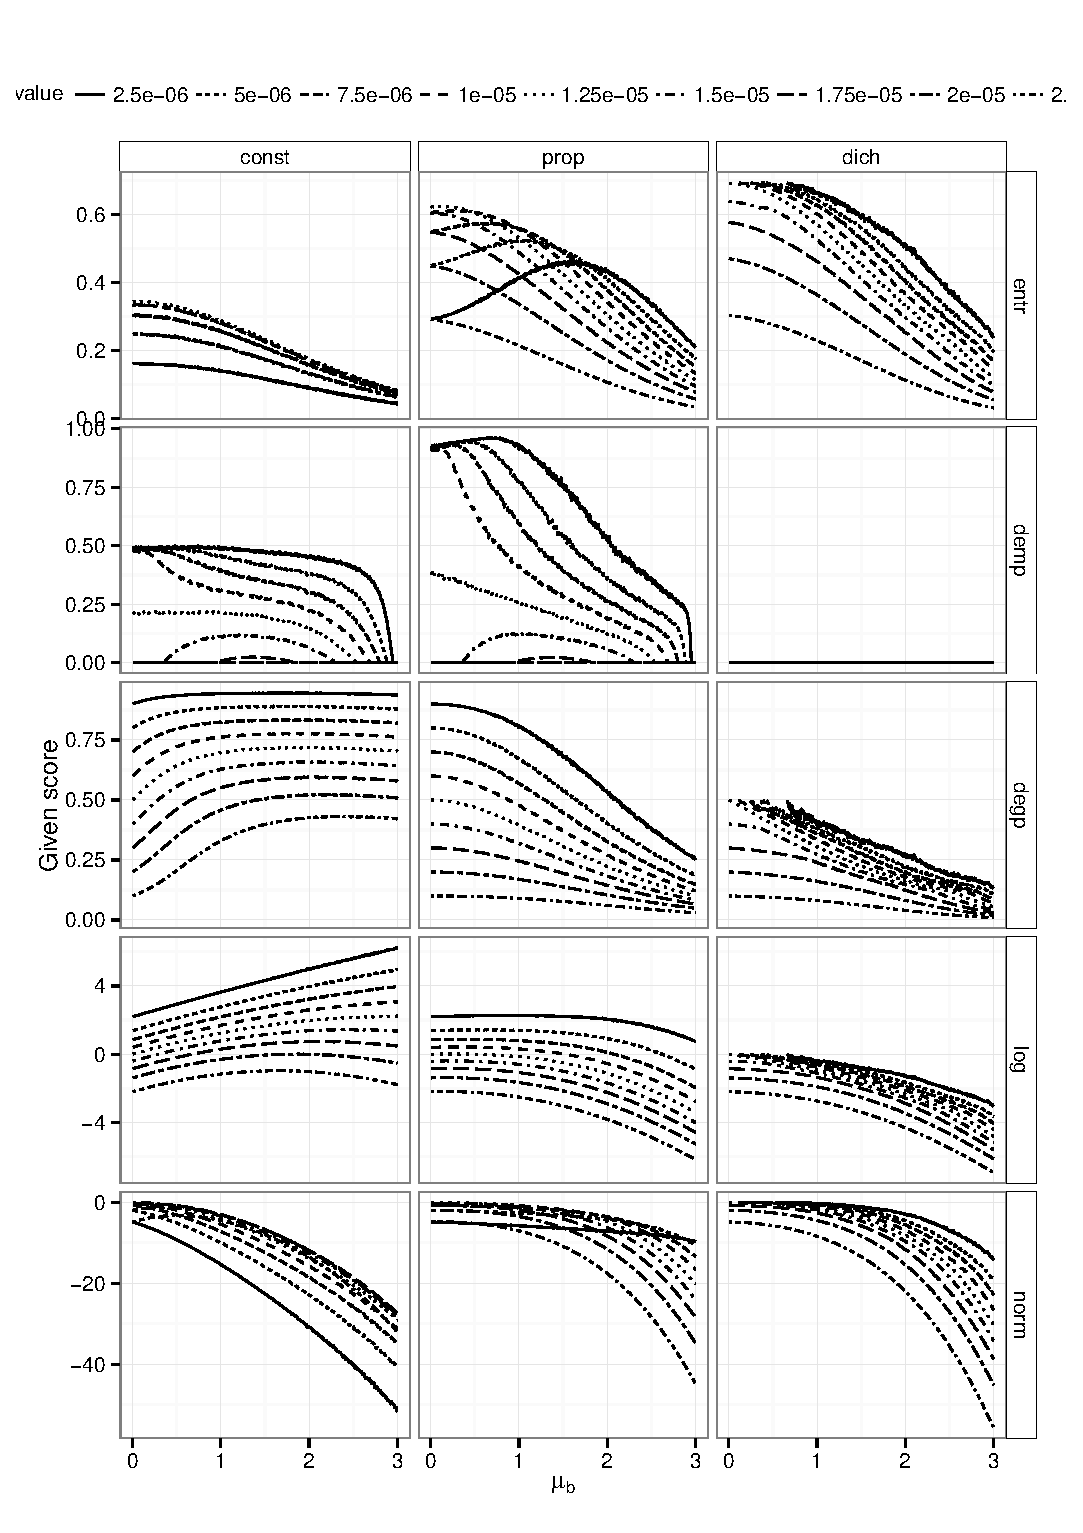
\includegraphics[scale=.5]{fig01ball.eps}
\caption{Score calculated for methods described for different approaches of $\lambda$ and $\omega$ score when $\mu_b$ varying}
\label{fig:mu_varying3}
\end{figure}


Now, the main difference between the results obtained in Figure~\ref{fig:mu_varying} and Figure~\ref{fig:mu_varying3} appear on the first column, which corresponds to those methods with the constant weighing function, i.e. $\omega(\hat{\m \tau}_{i \mathcal{I}_s}, a) = const$. {\color{blue} Alguna explicaci\'{o} de perqu\`{e} passa aix\`{o}?}

In each simulation, the second and third column scores the confusion between components similarly. Note that by construction, when the confusion between part $I_a$ and part $I_b$ is calculated with function $\lambda(\hat{\m \tau}_{i \mathcal{I}_s}, a, b)$, methods $DEGP$, $LOG$ and $LOG^2$ score the same whenever the ratio $\frac{\pi_a}{(1 - \pi_a)}$ and $\frac{\pi_a}{(0.5 - \pi_a)}$ is the same for mixture $f_2$ and $f_3$ respectively.


\subsection{Simulation example}

In this section we have generated different samples to test the performance of methods available at Table~\ref{table_methods}. To simulate our data sets we have used the R package MixSim~\citep{Citar mixxim} {\color{blue} falta la cita!!!}. This package allows us to generate mixtures with a fixed overlapping level, $\hat{\omega}$ {\color{blue} unificar notaci\'{o}. Aqu\'{\i} poses un hat a la omega, a la secci\'{o} 2 o b\'{e} la dones sense hat o b\'{e} amb un check}. The overlapping level $\hat{\omega}$ is a measure of how easy is to confuse two components. In fact,  $\hat{\omega}$ is measured as a probability an therefore it ranges between $0$ and $1$. In Figure~\ref{omega} three different samples coming from three different randomly generated mixtures with overlapping parameters  $\hat{\omega}=0.05$, $\hat{\omega}=0.25$ and $\hat{\omega}=0.45$ are shown.

\begin{figure}[!t]
\centering
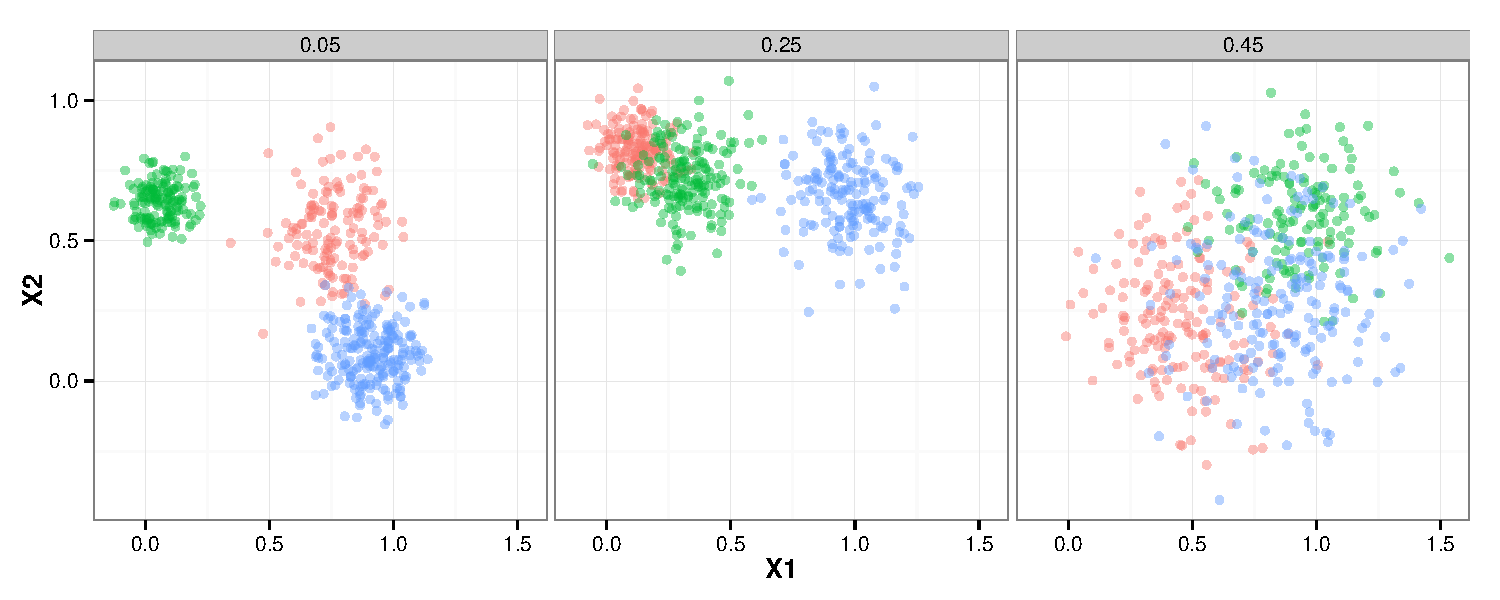
\includegraphics[scale=.5]{omega.pdf}
\caption{Example for different values of parameter $\hat{\omega}$}
\label{omega}
\end{figure}


For different values of $\hat{\omega}$ from $0$ to $0.5$ and each method $\mathcal{M}$ from Table~\ref{table_methods},  we  have repeated $1000$ times the following process:
\begin{enumerate}
\item Generate a sample $X$ of size $n=500$ with $D=5$ coordinates coming from a gaussian mixture with $3$ components whose components have maximum overlapping $\omega$. We keep the component which originates each element of sample $X$. Therefore, we have an original partition to which compare.
\item Fit a mixture with 9 components to sample $X$.
\item Using method $\mathcal{M}$ we have built a hierarchical partition as the one shown in Figure~\ref{hierarchical}.
\item We compare the original partition with the one obtained with method $\mathcal{M}$ at level $3$. To compare the similarity between the original partition and the one obtained in this step, we have used different indices. Because the overall results changed slightly, we have decided to show only one measure of similarity, the Agreement proportion. The Agreement proportion varies between $0$ and $1$, being $1$ a perfect agreement.
\end{enumerate}

Finally, we average the Agreement proportion obtained in the $1000$ simulations.

To compare the performance of presented methods, we have included a method which at step $3$ decides randomly the two components to merge. In Figure~\ref{fig:mub} we have plotted the obtained results. We have separated the methods depending on the weighing function.

In Figure~\ref{fig:mub} left, we have represented the methods which use the constant weighing function $\omega(\hat{\m \tau}_{i \mathcal{I}_s}, a) = const$. For lower levels of overlapping, the Entropy method (\cite{baudry2010combining}) is the one performing better. For higher level of overlapping, the $LOG_2$ and $DEGP$ methods perform slightly better than the others. This is coherent with the graphics shown in Figure~\ref{fig:mu_varying3} where those two methods were the only methods (with constant weighing) decreasing as the distance between distributions increased.

In Figure~\ref{fig:mub} center, we have represented the methods weighing the score by the posterior probability of begin generated by component $\hat{f}_{I_a}$, $\omega(\hat{\m \tau}_{i \mathcal{I}_s}, a) =  \hat{\tau}_{iI_a}$. All methods perform similarly in comparison to the ones which constant weighing function. Between them, the ones with higher agreement proportion are $LOG$ and $LOG^2$ performing almost equally, the one with lower agreement proportion is the $DEMP$ algorithm \citep{hennig2010methods}.

Finally, in Figure~\ref{fig:mub} right, we have represented the methods with dichotomic weighing function. The variation for all those methods is minimum. Remember that, in this case, the $DEMP$ method is of no use.

\section{Conclusions}
\label{conclusions}

\begin{figure}[!h]
\centering
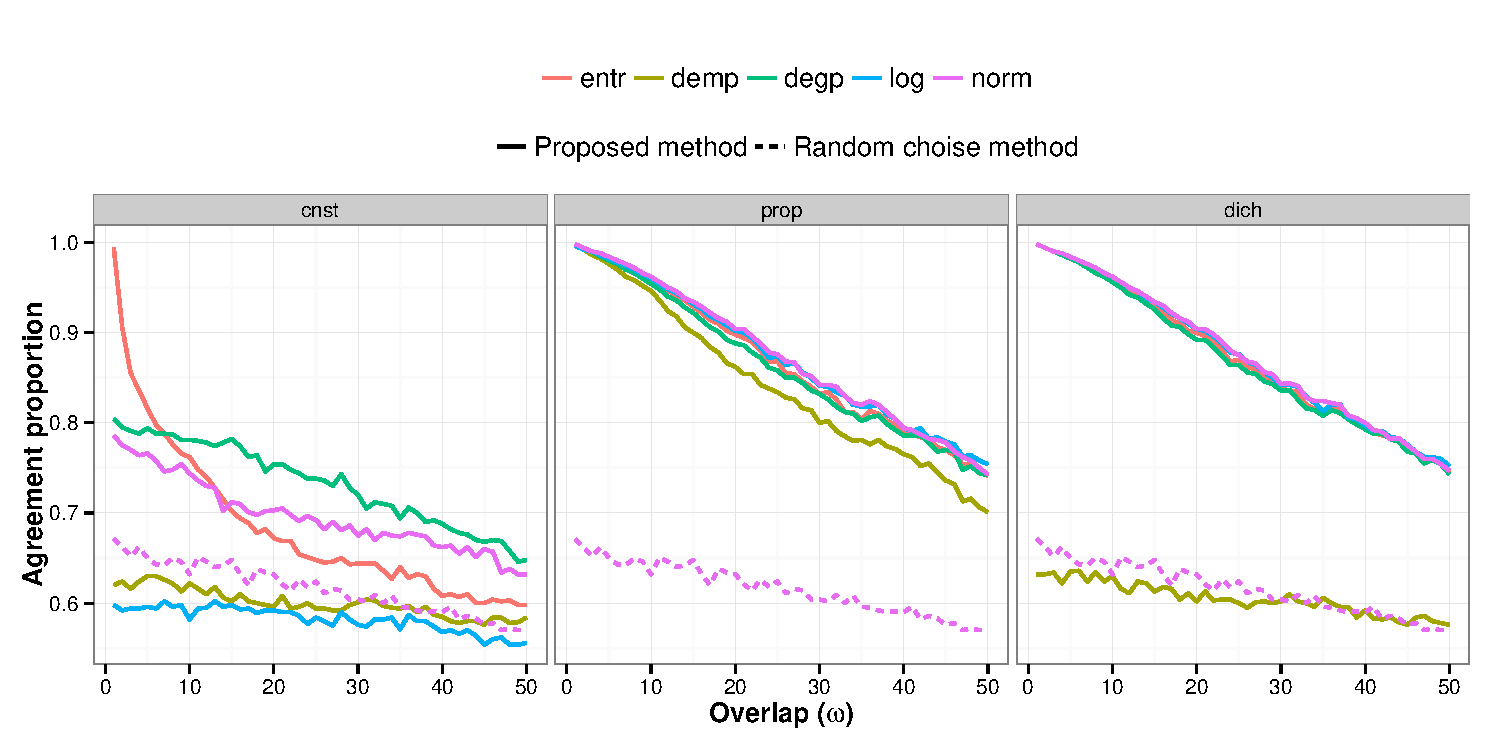
\includegraphics[width=\textwidth]{linesagreement.pdf}
\caption{$\lambda$ Agreement proportion results.}
\label{fig:mub}
\end{figure}


\bibliographystyle{apalike}
\begin{thebibliography}{}

\bibitem[Aitchison, 1986]{aitchison1986statistical}
Aitchison, J. (1986).
\newblock {\em {The Statistical Analysis of Compositional Data}}.
\newblock Monographs on Statistics and Applied Probability. Chapman \& Hall
  Ltd., London (UK).

\bibitem[Aitchison, 2002]{aitchison2002simplicial}
Aitchison, J. (2002).
\newblock {\em {Simplicial inference}}.
\newblock {\em Algebraic Methods in Statistics anb Probability}, 287: 1--22.

\bibitem[Baudry et~al., 2010]{baudry2010combining}
Baudry, J.-P., Raftery, A.~E., Celeux, G., Lo, K., and Gottardo, R. (2010).
\newblock {Combining Mixture Components for Clustering}.

\bibitem[Hennig, 2010]{hennig2010methods}
Hennig, C. (2010).
\newblock {Methods for merging Gaussian mixture components}.
\newblock {\em Advances in Data Analysis and Classification}, 4(1):3--34.

\bibitem[Lee and Cho, 2004]{lee2004combining}
Lee, H.-j. and Cho, S. (2004).
\newblock {Combining Gaussian Mixture Models}.
\newblock In Yang, Z., Yin, H., and Everson, R., editors, {\em Intelligent Data
  Engineering and Automated Learning – IDEAL 2004 SE - 98}, volume 3177 of
  {\em Lecture Notes in Computer Science}, pages 666--671. Springer Berlin
  Heidelberg.

\bibitem[Longford and Bartosova, 2014]{longford2014}
Longford, N.~T. and Bartosova, J. (2014).
\newblock {A confusion index for measuring separation and clustering}.
\newblock {\em Statistical Modelling}, 14(3):229--255.

\bibitem[Melnykov, 2013]{melnykov2013distribution}
Melnykov, V. (2013).
\newblock {On the Distribution of Posterior Probabilities in Finite Mixture
  Models with Application in Clustering}.
\newblock {\em Journal of Multivariate Analysis}, 122:175--189.

\bibitem[Pastore and Tonellato, 2013]{pastore2013merging}
Pastore, A. and Tonellato, S.~F. (2013).
\newblock {A Merging Algorithm for Gaussian Mixture Components}.
\newblock {\em SSRN Electronic Journal}, (04).

\end{thebibliography}


\end{document}
